\documentclass[12pt]{article}

\usepackage{graphicx}
\usepackage{fancyhdr}
\usepackage{rotating}
\usepackage{xcolor}
\usepackage{listings}
\usepackage{indentfirst}
\usepackage{float}
\usepackage[margin=1in]{geometry}


\setlength{\parskip}{\baselineskip}%

\lstset{basicstyle=\ttfamily,
  showstringspaces=false,
  commentstyle=\color{red}
  keywordstyle=\color{blue}
}

\title{CS 751: Introduction to Digital Libraries - Assignment 1}
\author{Jessica McConnell}
\date{\today}

\begin{document}
\maketitle

\section{Q1}

We were required to get 10,000 tweets, map the links in each tweet, get the headers for each link, determine the unique and duplicate URIs and build a histogram of redirects and HTTP status codes.

\subsection{Getting the tweets and headers}

I started my script for getting tweets by using the code provided at http://thomassileo.com/blog/2013/01/25/using-twitter-rest-api-v1-dot-1-with-python/ for twitter connectivity.  I then customized it to pull tweets, extract the creation date and links from the tweet, filter for content and get the headers for the links within the tweet.  I chose to use the search/tweets API to ensure I had a myriad of different topics and links in the tweets I pulled.

For each word in my wordlist the tweets.py script would perform a search returning the maximum of 100 tweets.  The script applied some filters to help ensure the returned tweets were not inappropriate and to check that the tweet had at least one link.  If the tweet did not pass the restrictions, the tweet was skipped.  I ended up having a wordlist of more than 2000 words to ensure I could get 10000 tweets.

After getting the links from the tweet, `tweets.py' uses subprocess to get all the headers by calling `curl -I \textit{link}'.

The URI count, tweet URIs, headers for the URIs and JSON from the tweet were saved for each tweet in the file `tweetsURI'.

\subsection{Final URIs}

I wrote a python script `finaluri.py' that reads through the `tweetsURI' file.  This script originally sets \textit{link} to the URI found in the tweet and then continues updating \textit{link} until it has reached the end of the headers for that URI.  It then checks to see if it is in the unique URI list.  If not, it is added to the unique URI list and the all URI list.  If it is, we add it to the duplicate URI list if it is not already in there and the all URI list.

The unique and duplicate URIs were outputted to the files `uniqueuri' and `dupuri' respectively.

URIs:\\
$\bullet$  All URIs: 10347\\
$\bullet$  Duplicate URIs: 1071\\
$\bullet$  Unique URIs: 7406

\subsection{Redirects}

I used a bash command to get the redirect code numbers from the headers.

\begin{lstlisting}[language=bash,caption={bash code}]
status=$(egrep ^HTTP/1.1 tweetsURI | cut -d' ' -f2- | egrep ^3)
lower=$(echo "$status" | tr '[:upper:]' '[:lower:]')
echo "$lower" | sort | uniq -c | sort -nr > redirects
\end{lstlisting}

Redirect Codes:\\
$\bullet$  19837 301 moved permanently\\
$\bullet$   1201 302 found\\
$\bullet$    540 302 moved temporarily\\
$\bullet$    208 303 see other\\
$\bullet$     95 301 ok\\
$\bullet$     21 307 temporary redirect\\
$\bullet$     15 302 object moved\\
$\bullet$     11 301 apple webobjects\\
$\bullet$      3 302\\
$\bullet$      2 301 www redirect\\
$\bullet$      2 301 movedpermanently\\
$\bullet$      1 302 please wait\\
$\bullet$      1 301 http://hee.nhs.uk/work-programmes/tel/hack\\
$\bullet$      1 301 found\\
$\bullet$      1 301

\begin{figure}[H]
    \centering
    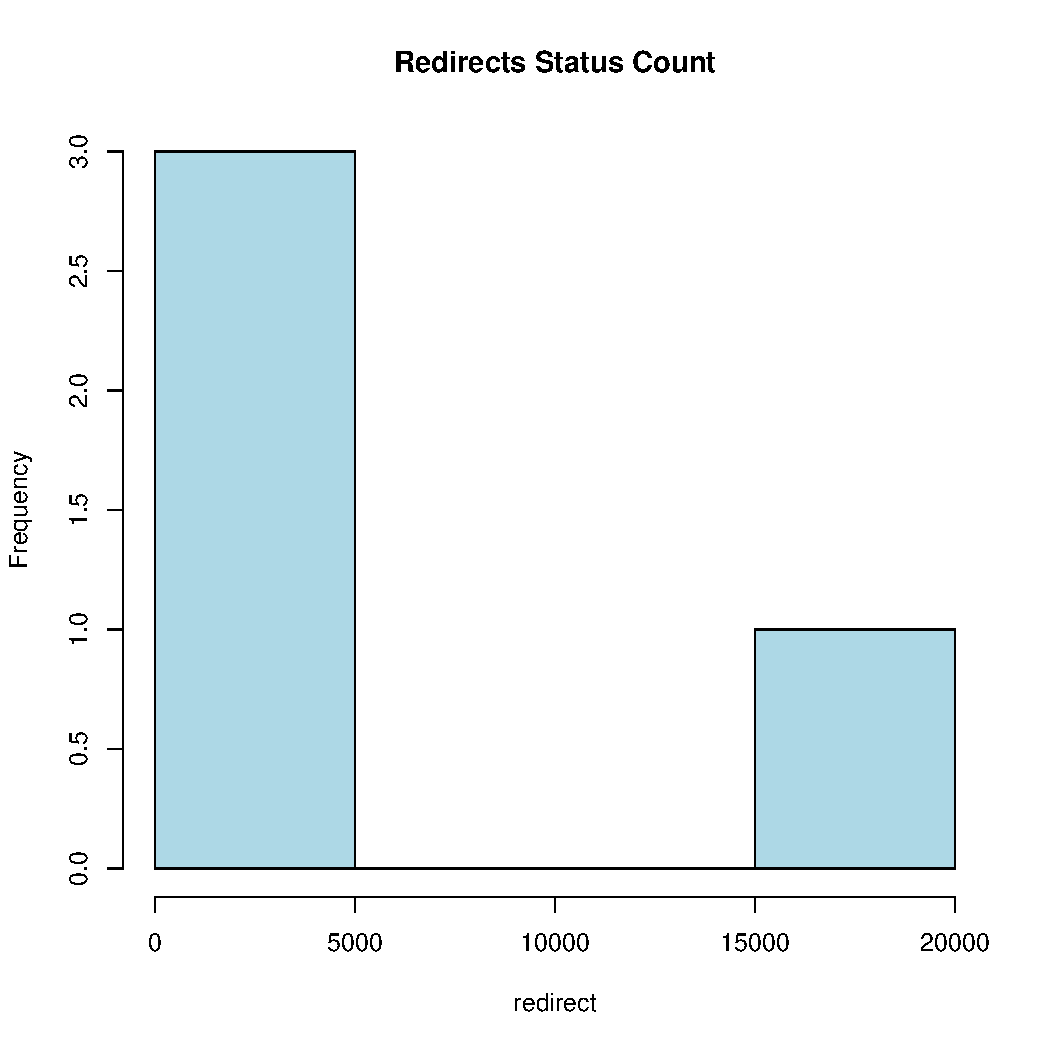
\includegraphics{redirectsPlot.pdf}
\end{figure}
NOTE: For the histogram I consolidated the above information into groups of individual code numbers instead of the specific textual responses.

\subsection{Status Codes}

I used a bash command to get the status code numbers from the headers.

\begin{lstlisting}[language=bash,caption={bash code}]
status=$(egrep ^HTTP/1.1 tweetsURI | cut -d' ' -f1,2)
echo "$status" | sort | uniq -c | sort -nr > statuses
\end{lstlisting}

Status codes:\\
$\bullet$  19949 HTTP/1.1 301\\
$\bullet$   9782 HTTP/1.1 200\\
$\bullet$   1757 HTTP/1.1 302\\
$\bullet$    208 HTTP/1.1 303\\
$\bullet$    191 HTTP/1.1 405\\
$\bullet$    107 HTTP/1.1 404\\
$\bullet$     47 HTTP/1.1 503\\
$\bullet$     46 HTTP/1.1 403\\
$\bullet$     42 HTTP/1.1 406\\
$\bullet$     21 HTTP/1.1 307\\
$\bullet$     16 HTTP/1.1 500\\
$\bullet$      7 HTTP/1.1 416\\
$\bullet$      3 HTTP/1.1 508\\
$\bullet$      3 HTTP/1.1 400\\
$\bullet$      3 HTTP/1.1 302\\
$\bullet$      1 HTTP/1.1 504\\
$\bullet$      1 HTTP/1.1 502\\
$\bullet$      1 HTTP/1.1 501\\
$\bullet$      1 HTTP/1.1 410\\
$\bullet$      1 HTTP/1.1 301\\
$\bullet$      1 HTTP/1.1 204

\begin{figure}[H]
    \centering
    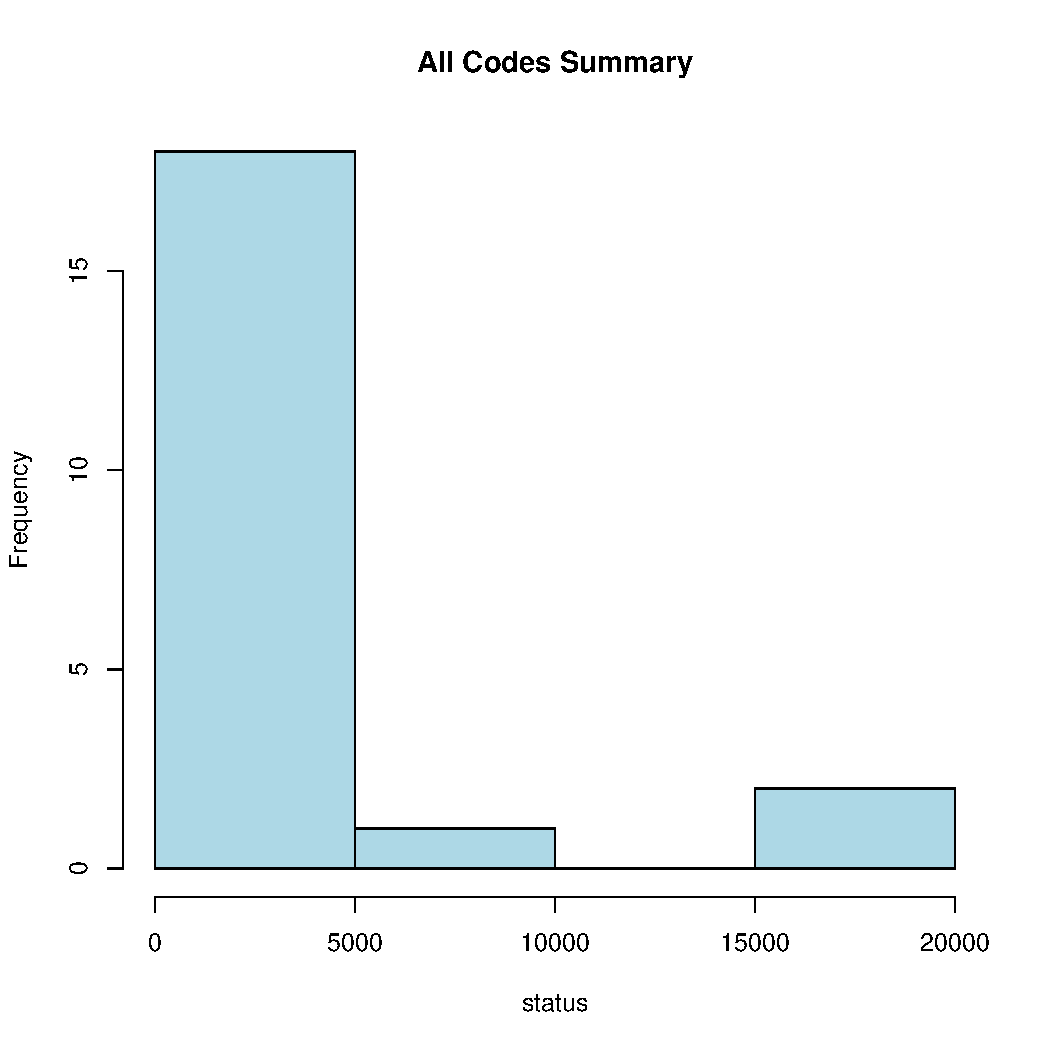
\includegraphics{statusCodesPlot.pdf}
\end{figure}
\section{Q2}

We were required to get the carbon date for all the links in the tweets, get the deltas between the age of the tweet and age of the link and perform statistical operations on the deltas.

\subsection{Running the Carbon Date Utility}

Since I had several duplicate URIs I decided to perform the carbon date on the final URIs instead of the links in the tweets directly.  I assigned each URI a number and created a directory for it in the carbondate directory.  Within the numbered directory for each individual URI I housed the results from `python local.py \textit{url}'.

I wrote two scripts to perform my carbon date lookups.  The main script is `getTimes.sh'.  It is called with the command found in `./getTimes.sh \textit{folder} \textit{url}'.  The script creates the numbered folder for the URI and calls `python local.py \textit{url}' outputting the results to \textit{folder}/cd.  The second script is called `getAll.sh'.  It is a wrapper script that calls the `getTimes.sh' script for each URI.

There were 4 URIs that were hung when I used my scripts.  I ended up using the carbon date utility provided at http://cd.cs.odu.edu/cd.  By doing this, I learned that they were having issues because some of the characters that were in the URIs.  I fixed this by changing the characters from ascii to url format.  For example: I changed ' to \%27.

\subsection{Determining the Deltas Between Tweet Age and Link Age}

I wrote a script called `addDatesToUri.py' that concatenated each URI and the date found to be earliest by the carbon date utility.  There were several URIs that I came across that had no dates in the response from carbon date and were skipped. The results were placed in a file called `uniqueuridates'.  The file ended up having 4345 entries with a date given from carbon date out of 7406 unique URIs.

To compute the difference in the ages I wrote a script named `timedif.py'.  This script starts by pulling in the information in `uniqueuridates'.  After that it begins to work through the tweetsURI file line by line.  If it sees a line that starts with CREATED\texttt{\_}AT: it changes the format of the date and saves it as \textit{tweetdate}.  If it sees a line that starts with URL or LOCATION, it saves the result in \textit{link}. Note this only saves the last one found before the end of the headers.  Once the script reaches the end of the headers for the twitter link, it searches for the final link in the list of known URIs.  If it is there, we perform a time difference between the \textit{tweetdate} and \textit{urldate}.  Otherwise, we make the time difference 0 and in doing this we say that twitter was the first known instance of the link.

\begin{figure}[H]
    \centering
    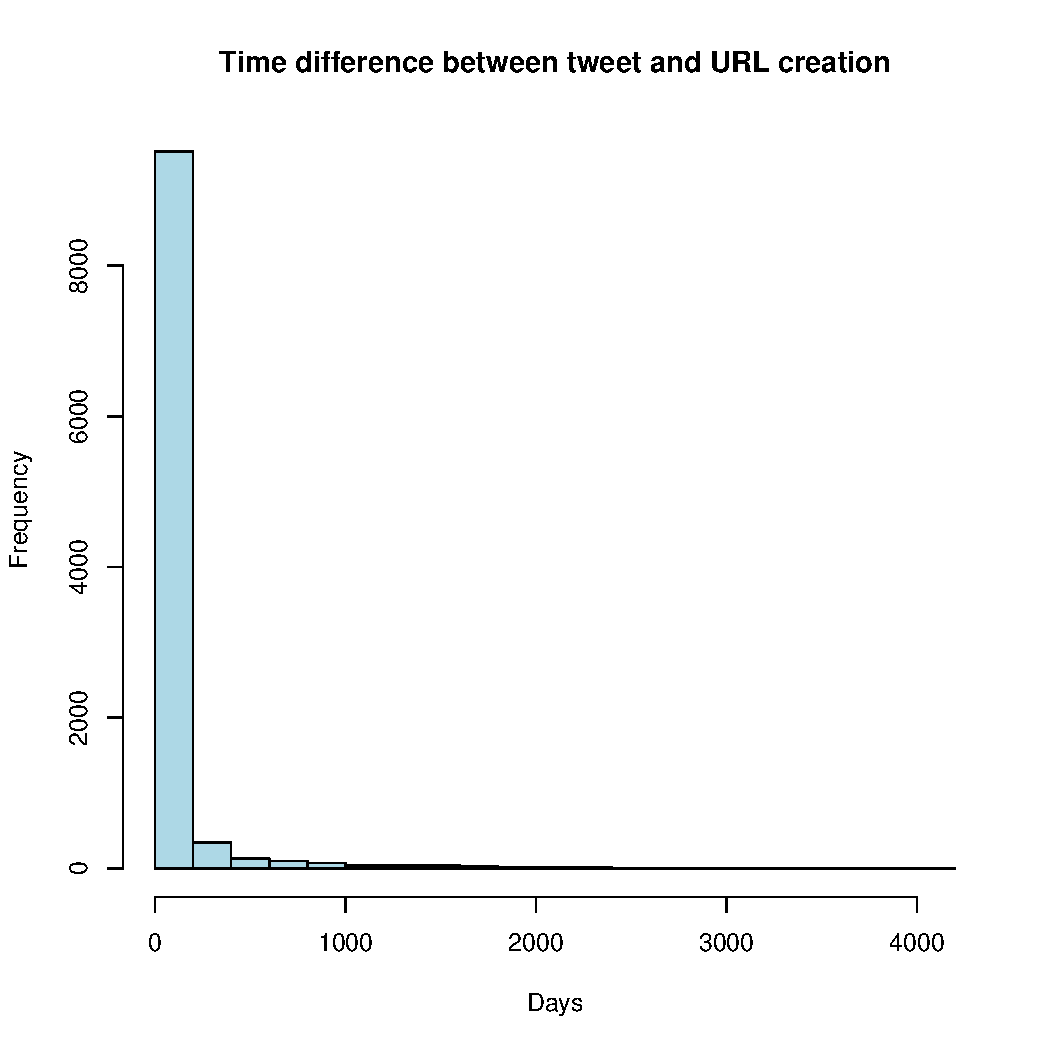
\includegraphics{timedif.pdf}
\end{figure}

\subsection{Statistics on Deltas}
I wrote a python program to perform my statistics operations named `time/stats.py'.  It returned the following information on my deltas.\\
$\bullet$ SUM:  690833\\
$\bullet$ NUMBER OF DELTAS:  10347\\
$\bullet$ MEAN OF ALL DELTAS:  66.76650236783608\\
$\bullet$ MEDIAN OF ALL DELTAS:  0\\
$\bullet$ STD ERR:  2.575788481411682\\
$\bullet$ STD DEV:  262.0097310333504\\

\end{document}
